%
%
%
\section{Self-consistent field procedure}

Central to solving the electronic structure problem using a basis set is finding solutions to the matrix eigenvalue problem, also known as the Roothaan equation

\begin{equation}
    \mat{H}\mat{C} = \mat{E}\mat{S}\mat{C}.
\end{equation}

The orthonormality relation among the plane waves simplifies the above expression to

\begin{equation}
    \mat{H}\mat{C} = \mat{E}\mat{C}.
    \label{eq:roothaan}
\end{equation}

as the overlap matrix $\mat{S}$ becomes the identity matrix. Despite this simplification, solving the above equation remains daunting due to the sheer number of basis functions (plane waves) involved, making these matrices very large. To illustrate this, consider a relatively small basis set size of 10,000 plane waves. Using double precision and noting that the matrix entries are complex-valued, each matrix would allocate a little under 1.5 GiB of memory.

Consider now the situation that we are basically only interested to find eigenvector and -values for only a relatively small number of Kohn-Sham states $N \ll N_{\textrm{pw}}$ roughly in the order of the number of electrons, i.e. the number of occupied states. In other words, solving \cref{eq:roothaan} in full is a waste of computational resources and would take an unnecessarily long time.

Fortunate for the field of computational chemistry (and many computational fields in general), there exist effective algorithms that allow one to only calculate a few eigenvector and -value pairs in a very large set. Furthermore, one can choose whether to find the lowest or highest eigenvalues in these algorithms. This aspect is important as only those eigenvectors that have the lowest eigenvalues are the most relevant in electronic structure calculations. The specific choice which method to use depends on the matrix properties such as symmetry or sparsity. For electronic structure calculations, the matrix $\mat{H}$ is typically sparse and diagonally dominant, making especially the Arnoldi\cite{1951:arnoldi} and Davidson\cite{1975:davidson} methods very effective. Within this work, we will focus on using the Arnoldi method as it is readily available in Scipy.\cite{arnoldi_scipy}

%
%
%
\subsection{Arnoldi method}

Using the Arnoldi method, one can approximate eigenvalues and eigenvectors of large, sparse matrices. The number of required eigenvector/-value pairs can be freely set and the method allows to focus on the lowest eigenvalues, i.e. those that are most relevant for the electronic structure calculation as unoccupied (virtual) Kohn-Sham states have no contributions to the total electronic energy.

Another strong feature of the Arnoldi method is that the Hamiltonian matrix $\mat{H}$ does not have to be explicitly known, only its effect when applied to an arbitrary vector $\vec{c}$ needs to be known, i.e. only a numerical procedure to calculate

\begin{equation}
    \vec{c}\;\prime = \mat{H}\vec{c}
\end{equation}

needs to be known. Using the plane wave basis set and the FFT to our advantage, this operation can be encapsulated as

\begin{equation}
    \hat{\mathcal{H}}\tilde{\psi}(\vec{G}) = \frac{1}{2} \hat{\mathcal{L}}\tilde{\psi}(\vec{G}) + \fftpw\left[\ifftpw\left[\tilde{\psi}(\vec{G}) \right] \circ \nu_{\text{eff}}(\vec{r}) \right]
    \label{eq:appl_hamil}
\end{equation}

where $\hat{\mathcal{L}}$ is the Laplacian operator, which when applied to the plane wave expansion of a Kohn-Sham state $\tilde{\psi}(\vec{G})$ yields

\begin{equation}
    \frac{1}{2} \hat{\mathcal{L}}\tilde{\psi}(\vec{G}) = \frac{1}{2} \cdot |\vec{G}|^{2} \circ \tilde{\psi}(\vec{G}).
    \label{eq:laplacian_applied}
\end{equation}

and where $\circ$ corresponds to the the Hadamard\footnote{The Hadamard product is simply the element-wise multiplication of two array-like objects. In \cref{eq:appl_hamil,eq:laplacian_applied}, $\tilde{\psi}(\vec{G})$ is a three-dimensional array of plane-wave coefficients. A Hadamard multiplication on $\tilde{\psi}(\vec{G})$ requires an array-like object of matching dimensions producing another array-like object of the same dimensions.} product operator. $\nu_{\text{eff}}(\vec{r})$ is the effective potential, which is the sum of the external, Hartree en exchange-correlation potentials as given by

\begin{equation}
    \nu_{\text{eff}}(\vec{r}) = \nu_{\text{ext}}(\vec{r}) + \nu_{U}(\vec{r}) + \nu_{\text{xc}}(\vec{r}).
\end{equation}

\cref{eq:appl_hamil} is counter-intuitive in the sense that first the plane-wave representation of the wave function $\psi(\vec{G})$ is first transformed to its real-space variant, after which the effective potential is applied to it (in real-space), after which the result is cast back to the plane wave representation. The sole reason for this is that the exchange-correlation functional is determined in real-space and involves a multiplication in real-space. This implies that its evaluation in the plane wave basis would require a very expensive convolution. Despite that it looks more convoluted\footnote{No pun intended.}, the sequence of operations as conducted in \cref{eq:appl_hamil} is computationally more efficient.

%
%
%
\subsection{Electron density mixing}

From the earlier section it was already established that $\nu_{\text{J}}[\rho]$ and $\nu_{\text{xc}}[\rho]$ depend on the electron density $\rho(\vec{r})$ and perhaps a more accurate way to write \cref{eq:roothaan} is

\begin{equation}
    \mat{H}[\rho]\mat{C} = \mat{E}\mat{C},
    \label{eq:roothaan_explicit}
\end{equation}

wherein $\rho$ in turn depends on the coefficient matrix $\mat{C}$ which encapsulates in its column space the plane wave expansion coefficients of the molecular orbitals $\psi_{j}$ such that

\begin{equation}
    C_{ij} = \tilde{\psi}_{j}(\vec{G}_{i})
\end{equation}

by which the electron density in real-space is calculated via

\begin{equation}
    \rho(\vec{r}) = 2\sum_{j}^{N_{\text{elec}} / 2} \left|\ifftpw \left[ \tilde{\psi}_{j}(\vec{G}) \right] \right|^{2}.
    \label{eq:edens}
\end{equation}

with $N_{\text{elec}}$ representing the total number of electrons in the system. Note that the specific form of \cref{eq:edens} implies that we assume a closed-shell system by which every molecular orbital (Kohn-Sham state) is doubly-occupied, i.e. hosting two electrons with opposite spin-orientation. It is further assumed that the set $\{ \psi_{j} \}$ is ordered from low to high energy such that the lowest states are occupied in line with the Aufbau principle.

\begin{Figure}
    \centering
    \resizebox{0.9 \textwidth}{!}{
        \tikzstyle{startstop} = [rectangle, rounded corners, minimum width=3cm, minimum height=1cm,text centered, draw=black, fill=black!90, text=white]
\tikzstyle{process} = [rectangle, minimum width=3cm, minimum height=1cm, text centered, draw=black, fill=black!10]
\tikzstyle{decision} = [diamond, minimum width=3cm, minimum height=1cm, text centered, draw=black, fill=black!80, text=white]
\tikzstyle{arrow} = [thick,->,>=stealth]

\begin{tikzpicture}[node distance=2cm]

\node (start) [startstop] {Start: Initial guess for $\rho$};
\node (process1) [process, below of=start] {Construct $\nu_{\text{J}}[\rho]$ and $\nu_{\text{xc}}[\rho]$};
\node (process2) [process, below of=process1, align=center] {Approximate lowest $N$\\Kohn-Sham states\\(Arnoldi method)};
\node (decision1) [decision, below of=process2, yshift=-1cm] {$\left\{\psi_{i}\right\}_{N}$ converged?};
\node (process3) [process, below of=decision1, yshift=-1cm] {Calculate $E_{\text{total}}$};
\node (decision2) [decision, below of=process3, yshift=-1cm] {$E_{\text{total}}$ converged?};
\node (process4) [process, right of=decision2, xshift=4cm] {Update $\rho$};
\node (process5) [process, right of=decision1, xshift=2cm] {Set $\psi_{0}$};

\node (stop) [startstop, below of=decision2, yshift=-1cm] {Done};

\draw [arrow] (start) -- (process1);
\draw [arrow] (process1) -- (process2);
\draw [arrow] (process2) -- (decision1);
\draw [arrow] (decision1) -- node[anchor=east] {Yes} (process3);
\draw [arrow] (process3) -- (decision2);
\draw [arrow] (process4) |- (process1);
\draw [arrow] (decision2) -- node[anchor=east] {Yes} (stop);
\draw [arrow] (decision2) -- node[anchor=north] {No} (process4);
\draw [arrow] (process5) |- (process2);
\draw [arrow] (decision1) -- node[anchor=north] {No} (process5);

\end{tikzpicture}
    }
    \captionof{figure}{Self-consistent field procedure within plane-wave density functional theory.}
    \label{fig:scf}
\end{Figure}

From \cref{eq:roothaan_explicit}, it becomes apparent that an iterative procedure to solve the electronic structure problem is required. The terms in the Hamiltonian $\hat{\mathcal{H}}$ depend on the electron density $\rho(\vec{r})$ which in turn depends on the plane wave expansion coefficients encapsulated in $\mat{C}$ which is the result of solving \cref{eq:roothaan_explicit}. In other words, we encounter the infamous chicken-egg problem. To resolve upon this dilemma, an self-consistent field approach is utilized wherein we start with an initial guess for $\rho(\vec{r})$, solve \cref{eq:roothaan_explicit}, and use the resulting $\mat{C}$ to construct an updated version of $\rho(\vec{r})$, by which we can repeat upon the procedure. We keep on performing these iterations until the electron density, or perhaps more elegantly the total electronic energy, no longer changes. A schematic overview of this procedure is shown in \cref{fig:scf}.

Besides this outer iterative procedure shown in \cref{fig:scf}, also an inner iterative procedure corresponding to the Arnoldi method is shown. The Arnoldi method itself is also iterative and in every cycle an improved set of eigenvectors is found. The accuracy of these eigenvectors and their associated eigenvalues can be assessed on the basis of the eigenproblem equation

\begin{equation}
    \mat{A} \vec{c}_{i} = \epsilon_{i} \vec{c}_{i}
\end{equation}

and only when the set of $\{ \vec{c} \}$ is compliant to the above equation, the inner loop is converged.

With respect to the outer iterative cycle, we can imagine a chain of electron densities $\rho_{i}$ that becomes with each iteration closer to the self-consistent field solution. To minimize upon the number of iterations required, it is advantageous to seek an optimal procedure to update $\rho$. It turns out that simply replacing the old $\rho$ with the updated one is not the most efficient as it can be result in ``overshooting''. To combat the ``overshooting'', one can slowly add the new $\rho$ to the old $\rho$ via

\begin{equation}
    \rho \leftarrow \alpha \rho_{\text{new}} + (1 - \alpha) \rho_{\text{old}}
\end{equation}

where $\alpha$ acts as a linear mixing constant. This type of linear mixing is the most simple one and more advanced mixing schemes exist.

%
%
%
\subsection{Solutions and visualization}

The solution to \cref{eq:roothaan} are the set of Kohn-Sham states that minimizes the total electronic energy. These Kohn-Sham states are colloquially known as the molecular orbitals. The wave function associated to these Kohn-Sham states are encoded in the column space of the matrix $\mat{C}$ using the plane wave basis set. Visualization of these molecular orbitals is fairly straightforward via application of \cref{eq:fft_pw_inverse}, yet there are two important things to note.

Since $\psi(\vec{r}): \mathbb{R}^{3} \rightarrow \mathbb{C}$, typical construction of contour plots or isosurfaces requires evaluation of both real and imaginary parts of $\psi(\vec{r})$. Furthermore, especially for isosurfaces, a relatively fine grid is needed. The sampling grid generated by \cref{eq:fft_pw_inverse} depends on the size of the basis set. As the size is typically kept to a minimum for the sake of computational efficiency, the sampling grid is relatively coarse.

To avoid having to sample both the real and imaginary part of the wave function, we can apply certain transformations to the wave function. These transformations should however keep the Kohn-Sham states orthonormal with respect to each other and should not affect the total electron density nor the kinetic energy of the states. Multiplying a wave function by a phase factor $\exp(i\varphi)$ will not change any of these properties.\footnote{Fundamentally speaking, one is also allowed to mix the occupied molecular orbitals among each other. This allows one to localize the molecular orbitals. We will not discuss such aspects here.} Thus, we can generate an equally valid new state from an existing one by a phase angle $\varphi \in [-\pi,\pi]$ such that

\begin{equation}
    \psi\prime(\vec{r}) \leftarrow \psi(\vec{r}) \cdot \exp \left(i \varphi \right).
    \label{eq:psi_transform}
\end{equation}

Observe that the operation in \cref{eq:psi_transform} always keeps the magnitude of the complex number conserved. Thus, its application will not affect the electron density corresponding to $\psi(\vec{r}_{i})$ and allows us to morph the complex scalar field to a real one. For our use case, we wish find the optimal $\varphi$ such that the sum of squares of the real part of the molecular orbital is maximized, i.e.

\begin{equation}
    \max_\varphi \left(\sum_{i}\mathfrak{R}\left[ \psi(\vec{r}_{i}) \cdot \exp \left(i \varphi \right)\right]^{2} \right).
    \label{eq:optimize_real}
\end{equation}

This is non-linear optimization problem and an efficient way to tackle this is to use the \texttt{differential\_evolution} method of Scipy.\cite{differential_evolution}

To address a suboptimal sampling size, upsampling techniques can be used. Perhaps the most elegant upsampling technique is one that makes use of the Fast Fourier Transform. Consider a Kohn-Sham state $\psi(\vec{r})_{[32]}$ as defined on a grid in real-space using 32 points per Cartesian direction. In reciprocal-space, the same wave function is represented by $\tilde{\psi}(\vec{G})_{[32]}$. To upsample the real-space grid, we first add to $\tilde{\psi}(\vec{G})_{[32]}$ additional plane wave vectors $\vec{G}\prime$, all with $\tilde{\psi}(\vec{G}\prime) = 0$. This process is sometimes called ``padding''. For this strategy to work, the new number of sampling points per Cartesian direction must be an integer multiple of the old number of sampling points. For example, we can choose to upsample the original molecular orbital by a factor of 4, yielding $\tilde{\psi}(\vec{G})_{[128]}$ in reciprocal-space.

Next, the coefficients $\tilde{\psi}(\vec{G})_{[128]}$ can be cast back to real-space using the inverse Fourier transform. Importantly, we have to be cautious about the fact that we have changed the number of sampling. \cref{eq:fft_pw_inverse} remains valid, but the constant $C_{t}$ has changed and we have to use adjust \cref{eq:ct} such that $N_{x},N_{y},N_{z}$ correspond to the new values. To put this in other words, if we have upsampled by a factor of 4, the constant $C_{t}$ decreases by a factor of $4^{3}=64$.

%
%
%
\subsubsection{Demonstration of phase-rotation for \ce{BH3}}

To demonstrate the principle of ``phase-rotation'' for visualization purposes, consider the \ce{BH3} molecule calculated in a $10 \times 10 \times 10$ \AA\; unit cell using 32 sampling points per Cartesian direction. The calculation is performed using the \texttt{PyPWDFT}\cite{pypwdft} program. In this demonstration, we will focus on the double-degenerate set of orbitals with $E$-symmetry, i.e. the third and fourth occupied molecular orbitals. In \cref{fig:bh3_before}, the electron density of $\psi_{3}$ and $\psi_{4}$ is sampled in the plane in which the \ce{BH3} molecule resides. For these settings, the calculation converges such that $\psi_{3}$ has a negligible imaginary component. Interestingly, the $\psi_{4}$ molecular orbital is smeared out over both real and imaginary domains. 

\begin{Figure}
    \centering
    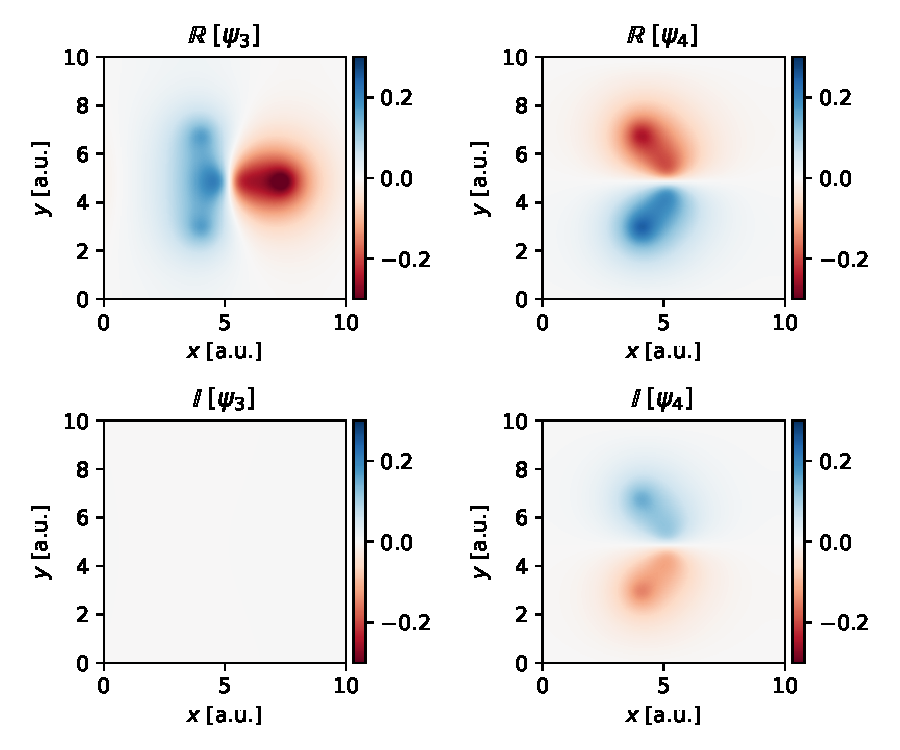
\includegraphics[width=\linewidth]{img/fig9.pdf}
    \captionof{figure}{Heat maps of the third and fourth occupied molecular orbital, i.e. the $E$-double-degenerate set, of the \ce{BH3} molecule. Top row corresponds to the real domain, bottom row to the imaginary domain. Note that $\psi_{4}$ has a non-negligible imaginary component.}
    \label{fig:bh3_before}
\end{Figure}

\begin{Table}
    \captionof{table}{Total amount of electron density, before and after a ``phase-rotation'' of $\varphi$, in the real domain for molecular orbitals $\psi_{3}$ and $\psi_{4}$ of the \ce{BH3} molecule. The value listed for $\varphi$ is the optimal angle (in degrees) that maximizes the real domain component.}
    \label{tab:phase-rotation}
    \centering
    \begin{tabular}{|c|r|r|r|}
        \hline
        \textbf{Orbital} & \(\varphi\) (deg) & \(\int_{\Omega} \mathfrak{R}\left[\psi\right]^{2} d\vec{r}\) & \(\int_{\Omega} \mathfrak{R}\left[\psi \cdot \exp(i \varphi)\right]^{2} d\vec{r}\) \\
        \hline
        $\psi_{3}$ & \texttt{0.0000} & \texttt{1.0000} & \texttt{1.0000} \\
        \hline
        $\psi_{4}$ & \texttt{31.1685} & \texttt{0.7321} & \texttt{1.0000} \\
        \hline
    \end{tabular}    
\end{Table}

\begin{Figure}
    \centering
    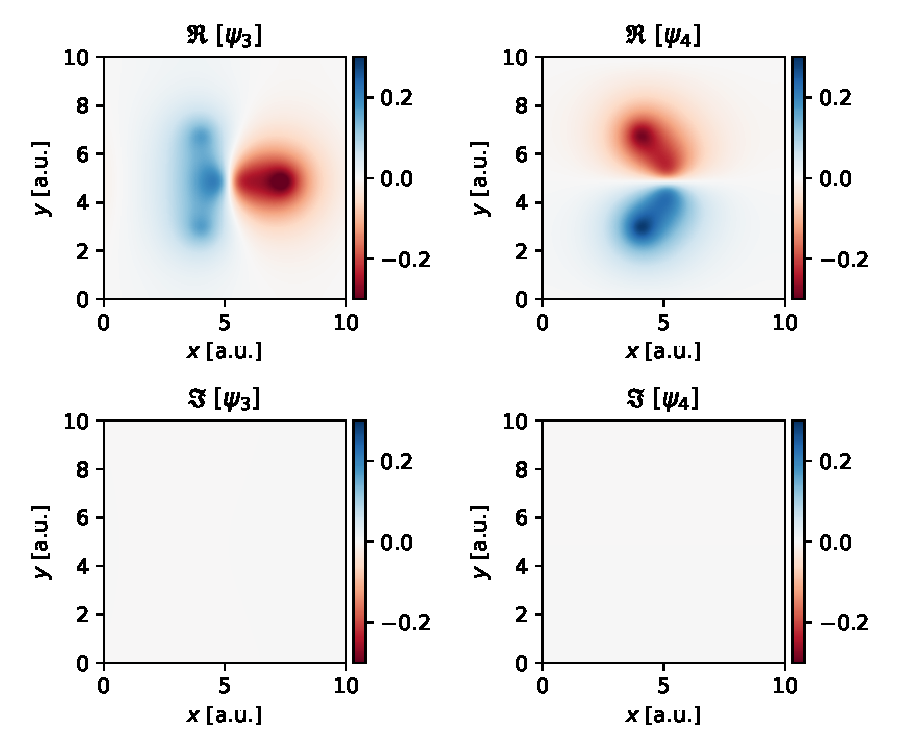
\includegraphics[width=\linewidth]{img/fig10.pdf}
    \captionof{figure}{Heat maps of the third and fourth occupied molecular orbital, i.e. the $E$-double-degenerate set, of the \ce{BH3} molecule after phase rotation. Top row corresponds to the real domain, bottom row to the imaginary domain. Note that the imaginary part of $\psi_{4}$ has become negligble.}
    \label{fig:bh3_after}
\end{Figure}

We now proceed to apply \cref{eq:optimize_real} to the two molecular orbitals with the aim of optimizing the real component of these orbitals by multiplication of a phase-factor $\exp \left(i \varphi \right)$. In \cref{tab:phase-rotation}, the total electron density for $\psi_{3}$ and $\psi_{4}$, prior and after this ``phase-rotation'', is provided. From this Table, it is clear that $\psi_{3}$ already has - within numerical approximation - all its electron density already in the real domain. In contrast, for $\psi_{4}$ only $\pm$73\% of its electron density resides in the real domain, the other $\pm$27\% in the imaginary domain.

By performing a ``phase-rotation'' using an angle of $\pm$31\textdegree, the imaginary part is rotated to the real domain, yielding a fully real-space molecular orbital. This is further reflected in \cref{fig:bh3_after}, where it can be seen that there are no more features found corresponding to the imaginary part.